\newpage
\section{Why Space Supervision Fails under Outcome Supervision?}
\label{app:c}

In Section~\ref{subsec:statealign}, we demonstrated that GR significantly enhances performance when paired with PS, serving as a semantic tether. However, a natural question arises: \textit{Can this semantic tethering mechanism independently rescue OS from its optimization barrier?}

Intuitively, one might hypothesize that the auxiliary reconstruction objective $\mathcal{L}_{\text{GR}}$ would inject rich semantic gradients into every latent state, thereby counteracting the "Gradient Attenuation" and "Primacy Bias" observed in the vanilla OS-LATENT baseline.

\paragraph{Empirical Failure.} 
Contrary to this intuition, experimental results (Table~\ref{tab:part1}) reveal that Space Supervision strategies fail to yield any meaningful improvement under the OS paradigm:OS-GC harms performance, confirming that imposing rigid geometric constraints on an unguided trajectory merely distorts the manifold.
Despite adding a decoder to enforce semantic content, the performance of \textsc{OS-GR} is indistinguishable from the trivial \textsc{OS-No-CoT} baseline and the vanilla \textsc{OS-LATENT}.

\paragraph{Mechanistic Analysis: The Persistence of Gradient Decay.}
To understand why the auxiliary reconstruction signal fails to correct the learning trajectory, we visualize the gradient norm distribution across latent positions for \textsc{OS-GR} versus the vanilla \textsc{OS-LATENT} baseline in Figure~\ref{fig:os_gradient_comparison}.

The visualization reveals a critical pathology: even with the auxiliary reconstruction loss, OS-GR (Left) exhibits a gradient distribution strikingly similar to the unaligned OS-LATENT (Right).
\begin{itemize}
    \item \textbf{Primacy Bias Persists:} In both settings, the first latent token $L_1$ dominates the gradient flow, while subsequent tokens ($L_2 \dots L_6$) suffer from decay.
    \item \textbf{Decoupled Optimization:} Although $\mathcal{L}_{\text{GR}}$ provides direct supervision to each $L_t$, these gradients function as \textit{local} alignment signals rather than \textit{global} reasoning signals. The model learns to encode just enough information in $L_t$ to satisfy the local reconstruction decoder to minimize $\mathcal{L}_{\text{GR}}$, but the main backbone continues to bypass these deep states for the final answer prediction $y$.
\end{itemize}

\begin{figure}[h]
    \small
    \centering
    \caption{\textbf{Gradient Norm Dynamics Comparison.} OS-GR exhibits a lower gradient magnitude than OS-LATENT. This indicates \textit{destructive interference} between the conflicting gradients of the local reconstruction objective and the global outcome shortcut, further proving the incompatibility of GR with pure Outcome Supervision.}
    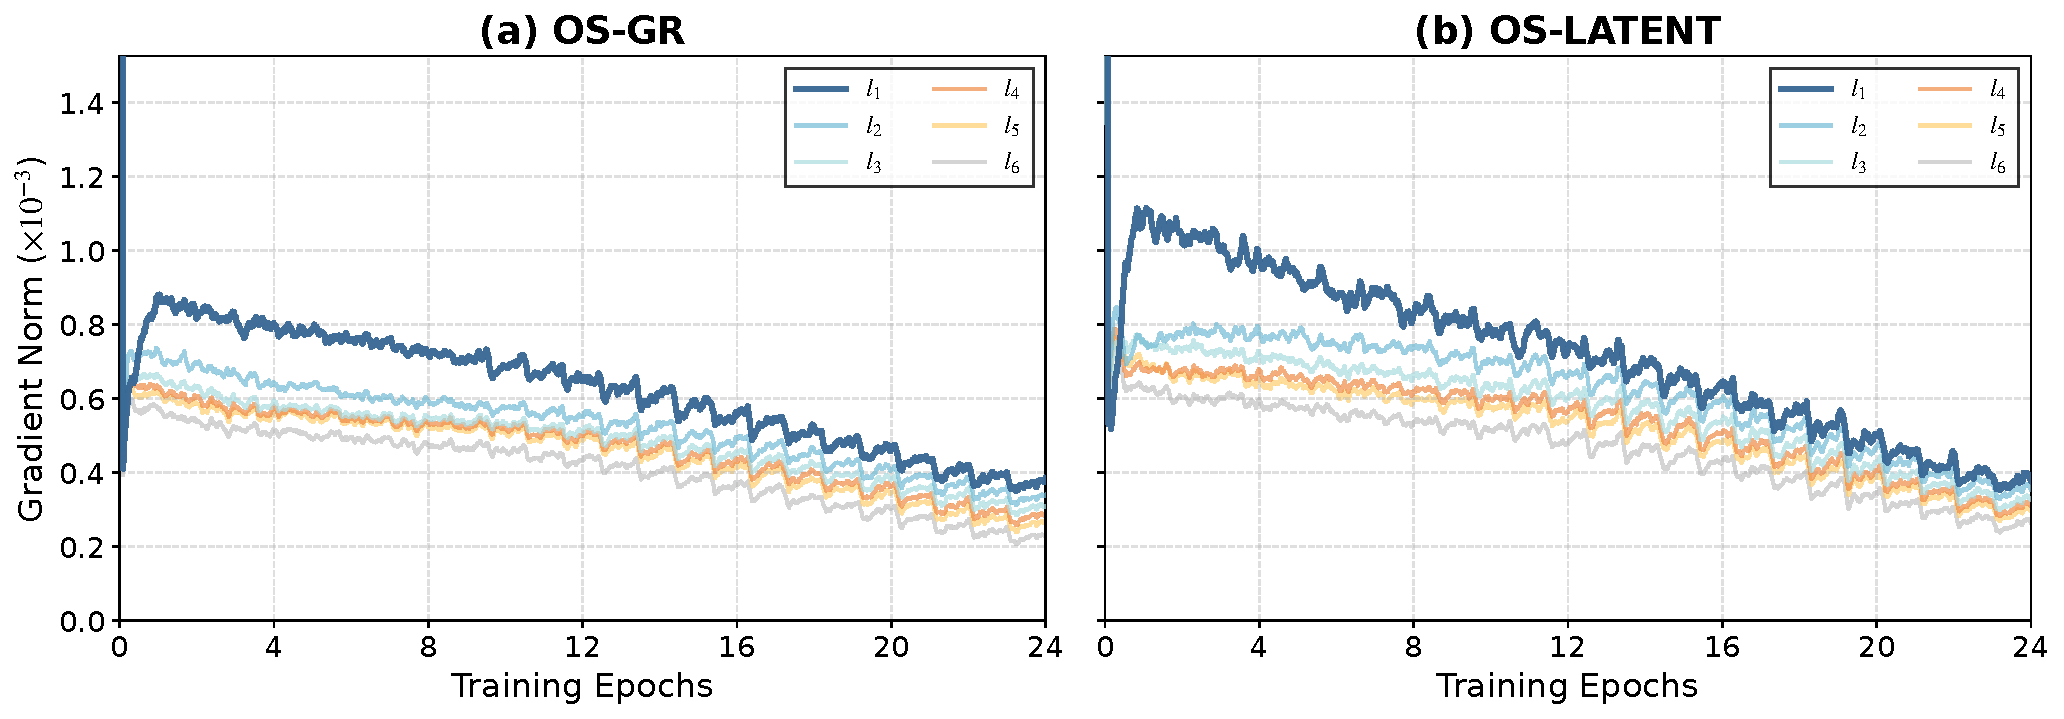
\includegraphics[width=\linewidth]{Figures/App/gradient_norms_compare.pdf} 
    \label{fig:os_gradient_comparison}
\end{figure}

This analysis highlights a fundamental theoretical distinction: \textbf{Space Supervision ensures semantic recoverability, but it does not guarantee causal utilization.} 
Without the Trajectory Scaffolding provided by Process Supervision to enforce the \textit{predictive} dependency $L_{t} \to L_{t+1}$, the model treats the latent states as isolated ``memory banks'' for reconstruction rather than steps in a coherent reasoning chain. Thus, structural scaffolding is the prerequisite for effective alignment.